\begin{chapter}{Proposed System}
    Machine translation is a field of natural language processing, it implies that computers translate one human-speaking language into another human-speaking language.

 Old methods of Machine translation include Rule-based, and statistical-based methods. Recently we have seen a rise in Deep Learning-based machine translation. Particularly, Transformer based models are very good in training with minimal human intervention. This system needs to get access to well aligned dataset. This is then it's feature learned by transformer based model.

In order to understand how to build a good machine translation system and how the system pipeline is structured. Most of these courses can be applied to basic natural language processing problems with the machine translation.

\textbf{Steps}

1. Data Collection

Parallel corpus is collected from various sources. It is possible to collect news texts, drama/movie subtitles, Wikipedia, etc., as well as data sets for evaluation of translation systems provided by WMT, a machine translation competition, and use them in translation systems. In our case, since our data is taken from OPUS Corpus. We select monolingual Malayalam files. Since those monolingual files are compressed files, we extract them to make them usable.

2. Cleaning

The collected data might have some quality issues, so they must be refined and cleaned. The refinement process includes sorting sentences by corpus in both parallel languages and eliminating noise such as unwanted extra spaces and special placing characters. Since we use OPUS Corpus as our initial data some level of quality is assured.

3. Subword Tokenization

Each NLP processing generally needs finely split units of input. Refine spacing and other alignment issues using natural language processing ie. NLP tools like the POS tagging tool or segmenting tool for each language. English may need refinement actions in  upper / lower case as data might be not properly cased in all cases. After the spacing is refined, use Byte Pair Encoding (BPE) using public tools such as SentencePiece , Subword or WordPiece. This allows you to perform additional segments and construct a dual-language vocabulary list. At this time, the segmented models learned for the BPE segment should be kept for future use.

4. Train

Training the seq2seq model with prepared parallel language datasets is needed. Depending on dataset amount preesent, you can train with one GPU, or use more than one GPUs in parallel to reduce training time. Parallel training usually improves the training time by a good margin. That's one reason we often go for GPU for training. GPU have more number of parallel processing cores. General Purpose Graphical Processing Units known as GPGPU is very common for training. The GPGPU from Nvidia and Google are quite popular.

5. Translate

Once training is completed, and the model has been created, you can start the translation with the model. Just provide well-formatted data as input, we get an output.

6. Detokenization

Even after the our transformer model based translation process is finished, the output is still in aj text segment, so it is not same as the data from the actual sentence structure used by real people. Thus, when you perform a detox process, it is returned in required form of the real sentence.

7. Evaluating

In order to evaluate our model performance, Quantitative evaluation is taken place on the sentence thus transliterated. BLEU is most popular  quantitative evaluation matrix for machine translation. You can decide which model is superior by comparing one model BLEU score with another model's BLEU score.

    \begin{section}{Dataset Preparation}
    Generally, translation systems need high-quality parallel data with a good variety of content. That means data should be available in source and target languages. And those two data should be well aligned with each other. Then only training with such a dataset provides a meaningful result to the training. We visit OPUS Corpus website and download appropriate file for training. In our case, Malayalam file is downloaded and processed with ml2en library by means of backtranslation.
    \end{section}

    \begin{section}{Proposed System}
    Our system utilizes highly performant PyTorch-based code that process our training data to produce a transliteration model. Moses file format is used for training. Moses files are simply well aligned files from both languages. How to deploy with CTranslate2.

    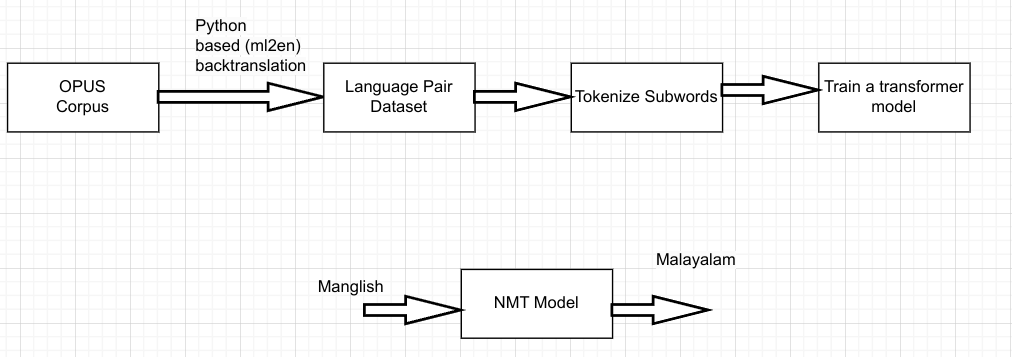
\includegraphics[width=\linewidth]{Images/proposed-system.png}

    As we can see in the above image, we need to backtranslate the data to build a dataset first. Then we need to split the data into minute possible representations of each word. That's how subwording and tokenization come into the picture. Once all our pre-processing is done, we can train the model. Once the model is built, we can reuse the same model any number of times we want. And Transformers are good at tracking sequence-to-sequence data.
    
    \end{section}

    \begin{section}{Toolbox}
    \begin{itemize}
        \item \textbf{Google Colab:} is a cloud-based coding tool for experimenting with ML / DL workloads. It's wire-compatible with award-winning Jupyter Notebooks or Jupyter Labs. That's why we are able to export with "*.ipynb" format. It provides access to CPU / GPU / TPU on demand. This GPU access make it easy to train the models.
       \item \textbf{Python:} is the best programming language for ML / DL workloads, since it's having a lot of good libraries and all.
        \item \textbf{ml2en:} is a library for converting from Malayalam to Manglish. This reverse translation data is used as the synthetic data for the algorithm. This might useing some rule-based logic as far as I can guess.
        \item \textbf{PyTorch:} a python library with various ML/DL functions. And its is very python interface built from ground for python. It was inspired by torch framework of LuaJIT language.
        \item \textbf{OpenNMT: } A library that implements highly optimized translation pipelines. Makes building translation or transliteration models very easy.
        \item \textbf{CTranslate2:} is a high-performance inference engine, which is used for inferring the output based on the model we build. Sometimes, we may need to convert the model to make it usable with CTranslate2.
        \item \textbf{StreamLit:} a framework that help data scientists to build interactive dashboards quickly. This doesn't need to know web development knowledge yet provides a Python-based workflow for making Python developer life easy by providing high-quality interactive widgets.
    \end{itemize}
    \end{section}

    \begin{section}{Implementation and Training} 
        As we mentioned before after the preparation of the dataset by means of backtranslation and all. We need to ensure training proper embeddings are learned.

        \subsection{Subwording}
        Since learning of embeddings is limited by the memory we have in our system we have to limit the vocabulary size. To do that we split words into subwords and keep the limit. But, subwords are not natural to our fellow humans. So we have to desubword after transliteration.

        \subsection{Learning Embeddings}
        This can be done by employing Byte Pair Encoding or Unigrams. As we know from our NLP knowledge, the words that come together have some sort of association. And the word surrounding it defines some meaning to the word itself. So from the SentencePiece transformer package, we can utilize any of the methods. I chose the unigram model since it was more conceptually familiar.

        \subsection{Training}
        After embeddings are learned we can finally proceed with model building. By training each possible embeddings are used to calculate the weights of the transformer. After enough number of training steps the model weights are written into a model file. These model weights are used for doing the actual translation afterward. Default value of our OpenNMT implementation was 10000 steps. After tweaking a little bit things here and there we were able to save a model into file. It was taking around 900MB in size, but after applying production level things it was reduced to around 300MB. 
        
    \end{section}
\end{chapter}